%!TEX root=paper.tex
\section{Method}\label{method}

Our method builds on the architecture described in \cite{Girshick2014}, summarized in \autoref{fig:rcnn}.

\begin{figure}[h!]
\begin{center}
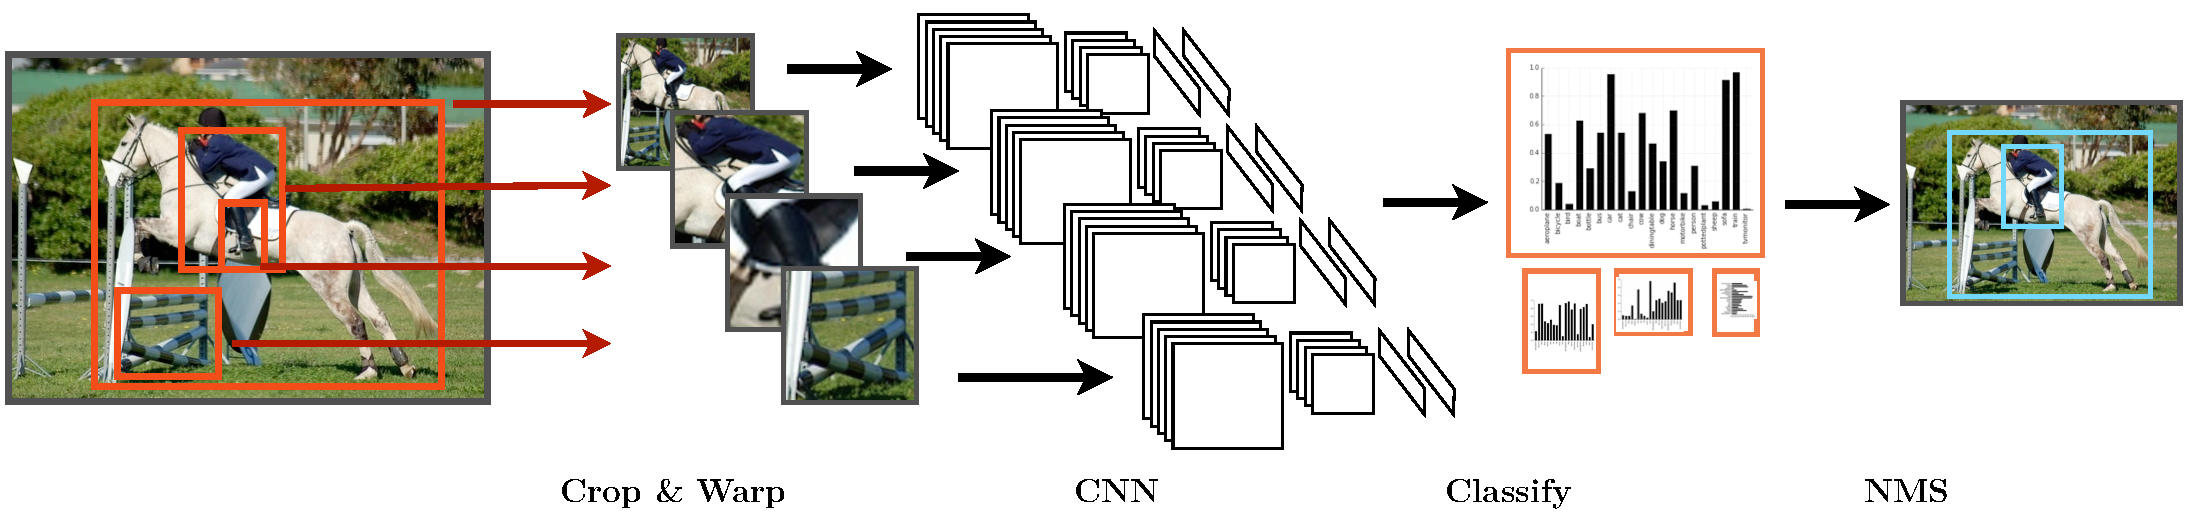
\includegraphics[width=0.98\columnwidth]{figures/rcnn.pdf}
\caption{
R-CNN architecture: image regions are cropped, resized, and each one fed through a CNN with classification layers.
The classifier outputs are post-processed to give the final detections.
}\label{fig:rcnn}
\end{center}
\end{figure}

%%%%%%%%%%%%%%%%%%%%%%%%%%%%%%%%%%%%%%%%%%%%%%%%%%%%%%%%%%%%%%%%%%%%%%%%%%%%%%%
\subsection{Dense region evaluation}\label{dense-region-evaluation}

\autoref{fig:dense_rcnn} shows the dense region evaluation.

\begin{itemize}
\itemsep1pt\parskip0pt\parsep0pt
\item
  Explain the difference between cropping pixels and cropping \texttt{pool5}.
\item
  Explain design choices (single vs multi scale, finding nearest window, warping.
\end{itemize}

\begin{figure}[h!]
\begin{center}
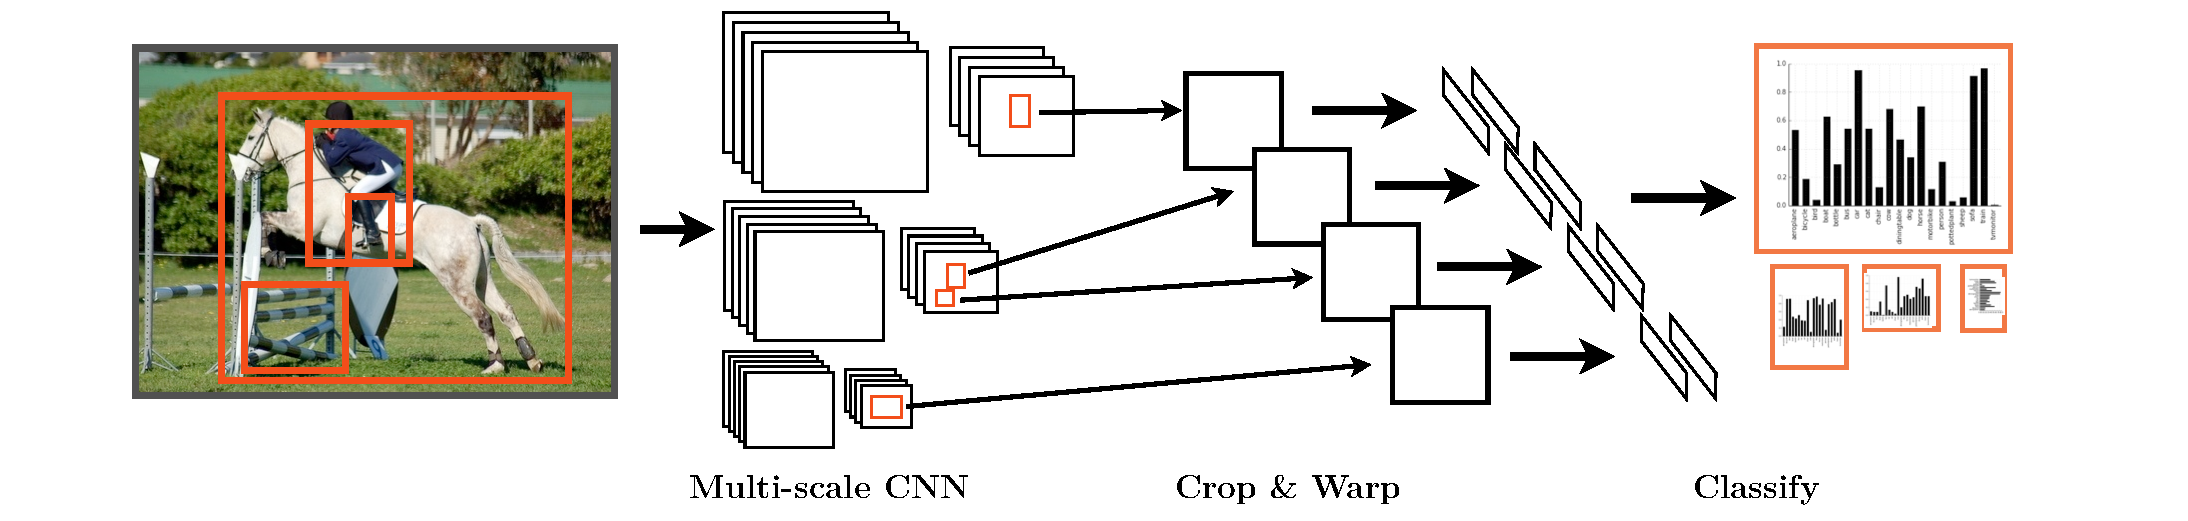
\includegraphics[width=0.98\columnwidth]{figures/dense_rcnn.pdf}
\caption{
Post R-CNN architecture: the whole image is fed through a CNN up to the highest pooling layer.
Regions are cropped from that layer, resized, and classified.
The classifier outputs are post-processed to give the final detections.
}\label{fig:dense_rcnn}
\end{center}
\end{figure}

%%%%%%%%%%%%%%%%%%%%%%%%%%%%%%%%%%%%%%%%%%%%%%%%%%%%%%%%%%%%%%%%%%%%%%%%%%%%%%%
\subsection{Cascaded CNN}\label{cascaded-cnn}

\begin{itemize}
\itemsep1pt\parskip0pt\parsep0pt
\item
  Explain the reject option in the CNN evaluation
\item
  Each rejector is trained to distiguish background regions from foreground (object) regions.
\item
  Explain training the thresholds
\item
  {[}FIGURE: Cascaded CNN, showing threshold layers{]}
\end{itemize}

%%%%%%%%%%%%%%%%%%%%%%%%%%%%%%%%%%%%%%%%%%%%%%%%%%%%%%%%%%%%%%%%%%%%%%%%%%%%%%%
\subsection{Dynamic region selection}\label{dynamic-region-selection}

\autoref{fig:combined} shows the dynamic region selection loop.

\begin{itemize}
\itemsep1pt\parskip0pt\parsep0pt
\item
  Explain dynamic selection of region batches
\item
  Explain iterative training procedure
\end{itemize}

\begin{figure}[h!]
\begin{center}
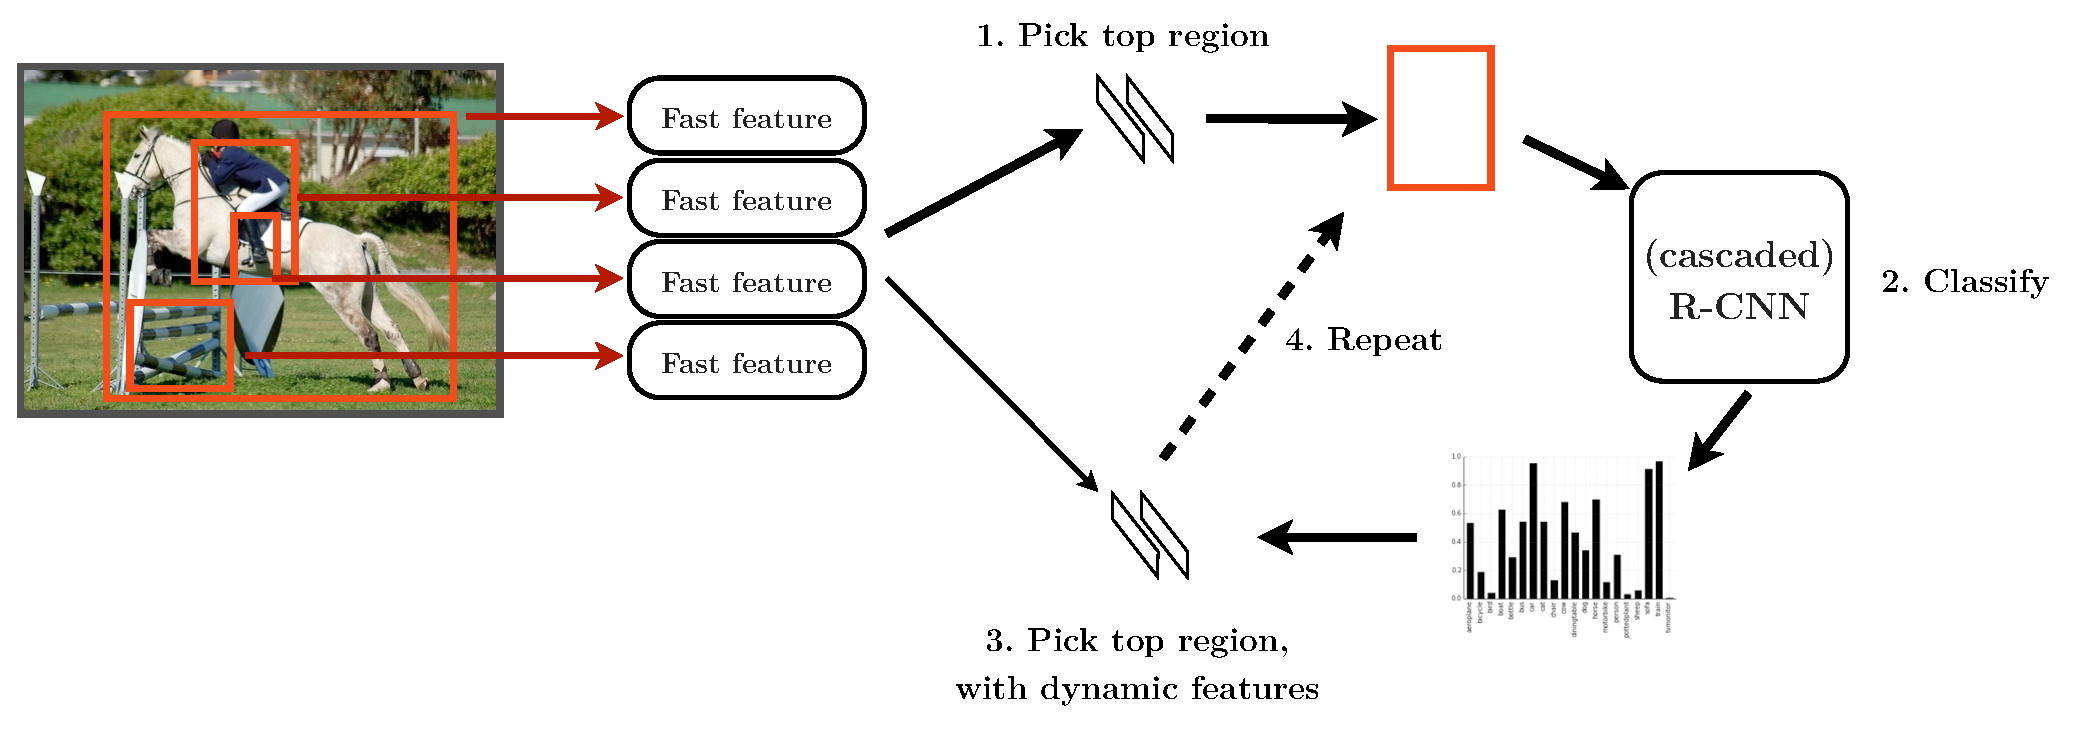
\includegraphics[width=0.98\columnwidth]{figures/combined.pdf}
\caption{
Dynamic region selection combines both speedups and introduces another.
}\label{fig:combined}
\end{center}
\end{figure}

%%%%%%%%%%%%%%%%%%%%%%%%%%%%%%%%%%%%%%%%%%%%%%%%%%%%%%%%%%%%%%%%%%%%%%%%%%%%%%%
\subsection{Combined system}\label{combined-system}

The entire system is combined by using Dense R-CNN as the fast feature and Cascaded CNN as the region evaluator in \autoref{fig:combined}.
